\documentclass
[
  draft    = true,
  fontsize = 11pt,
  parskip  = half,
  BCOR     = 0pt,
  DIV      = calc,
  ngerman,
  usenames,
  dvipsnames
]
{scrartcl}

\usepackage[utf8]{inputenc}
\usepackage[T1]{fontenc}
\usepackage{lmodern}
\usepackage{babel}
\usepackage{amsmath}
\usepackage{amssymb}
\usepackage{tikz}
\usepackage{xcolor}
\usepackage{siunitx}

% Das Zeichen := in einer zentrierten Version
\mathchardef\ordinarycolon\mathcode`\:
\mathcode`\:=\string"8000
\begingroup \catcode`\:=\active
  \gdef:{\mathrel{\mathop\ordinarycolon}}
\endgroup

\pagestyle{empty}

% ------------------------------------------------------------------------------
\begin{document}
% ------------------------------------------------------------------------------

% height of a fraction in displaystyle
\newsavebox{\dummy}%
\sbox{\dummy}{$\displaystyle\frac{b}{a}$}%
\newlength{\ruled}%
\setlength{\ruled}{\dp\dummy}%
\newlength{\rulet}%
\setlength{\rulet}{\ruled}%
\addtolength{\rulet}{\ht\dummy}%
\newcommand{\colgap}{\rule[-\ruled]{0pt}{\rulet}\quad}%

\enlargethispage{3\baselineskip}

% -------------------------------------------------------
\section*{Grafische Lösung einer quadratischen Gleichung}
% -------------------------------------------------------
Eine quadratische Gleichung \emph{grafisch} zu lösen bedeutet, dass man die
Schnittpunkte zwischen einer Geraden und der Normalparabel konstruieren muss.
\begin{alignat*}{3}
                 &\colgap &     y&=ax^2+bx+c                   & \qquad&\vert-ax^2\quad\vert-y \\
  \Leftrightarrow&\colgap & -ax^2&=bx+c-y                      & \qquad&\vert:(-a)             \\
  \Leftrightarrow&\colgap &   x^2&=-\frac{b}{a}x+\frac{y-c}{a} & \qquad&\vert\;m:=-\frac{b}{a}\quad\vert\;n:=\frac{y-c}{a} \\
  \Leftrightarrow&\colgap &   x^2&=mx+n                        & \qquad&
\end{alignat*}

% ------------------
\paragraph{Beispiel}
% ------------------
Gesucht werden die Nullstellen der Funktion $f(x)=x^2-x-2$,
also die Lösungen der Gleichung $0=x^2-x-2$.

Dazu formt man die Gleichung zunächst so um, dass der quadratische
Teil mit Koeffizient 1 allein auf einer Seite steht:
\begin{equation*}
  0=x^2-x-2\qquad\Leftrightarrow\qquad x^2=x+2
\end{equation*}

Nun zeichnet man die Normalparabel $y=x^2$ und die Gerade $y=x+2$ in ein
Koordinatensystem. Die $x$-Koordinaten der beiden Schnittpunkte sind die
gesuchten Lösungen: $x_1=-1$ und $x_2=2$.
\begin{center}
  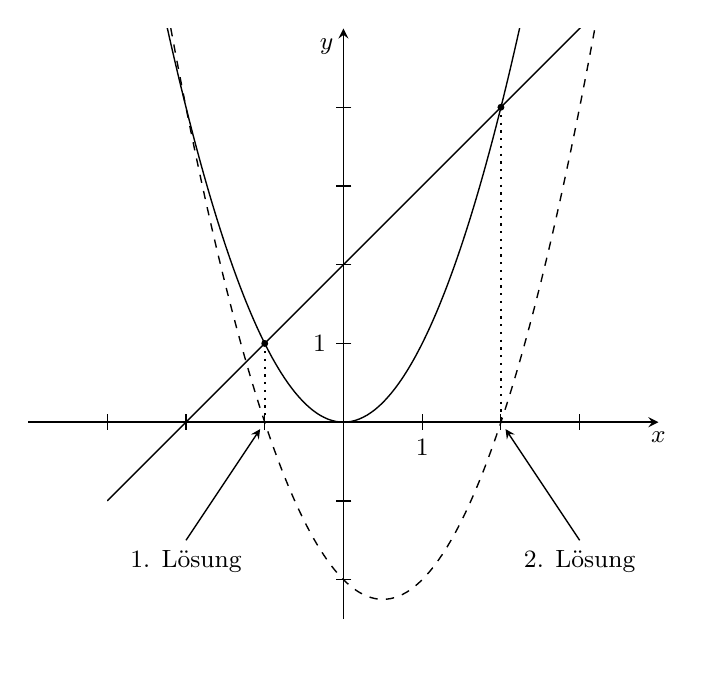
\begin{tikzpicture}
    % Koordinatenachsen
    \draw[line width=0.6pt, ->, >=stealth] (-4, 0) -- (4, 0) node[below] {{\small$x$}};
    \draw[line width=0.6pt, ->, >=stealth] (0, -2.5) -- (0, 5) node[below left] {{\small$y$}};
    % Skalierung der x-Achse
    \draw[xshift=-3cm] (0, 0.1) -- (0, -0.1);
    \draw[xshift=-2cm] (0, 0.1) -- (0, -0.1);
    \draw[xshift=-1cm] (0, 0.1) -- (0, -0.1);
    \draw[xshift= 1cm] (0, 0.1) -- (0, -0.1) node[below]{{\small$1$}};
    \draw[xshift= 2cm] (0, 0.1) -- (0, -0.1);
    \draw[xshift= 3cm] (0, 0.1) -- (0, -0.1);
    % Skalierung der y-Achse
    \draw[yshift=-2cm] (0.1, 0) -- (-0.1, 0);
    \draw[yshift=-1cm] (0.1, 0) -- (-0.1, 0);
    \draw[yshift= 1cm] (0.1, 0) -- (-0.1, 0) node[left]{{\small$1$}};
    \draw[yshift= 2cm] (0.1, 0) -- (-0.1, 0);
    \draw[yshift= 3cm] (0.1, 0) -- (-0.1, 0);
    \draw[yshift= 4cm] (0.1, 0) -- (-0.1, 0);
    % Graphen
    \begin{scope}
      \clip (-3.000, -3.000) rectangle (4.000, 5.000);
      \draw[line width=0.5pt, style=dashed] plot[smooth] coordinates
      {
        ( -3.000,  10.000)	        ( -2.900,   9.310)
        ( -2.800,   8.640)	        ( -2.700,   7.990)
        ( -2.600,   7.360)	        ( -2.500,   6.750)
        ( -2.400,   6.160)	        ( -2.300,   5.590)
        ( -2.200,   5.040)	        ( -2.100,   4.510)
        ( -2.000,   4.000)	        ( -1.900,   3.510)
        ( -1.800,   3.040)	        ( -1.700,   2.590)
        ( -1.600,   2.160)	        ( -1.500,   1.750)
        ( -1.400,   1.360)	        ( -1.300,   0.990)
        ( -1.200,   0.640)	        ( -1.100,   0.310)
        ( -1.000,   0.000)	        ( -0.900,  -0.290)
        ( -0.800,  -0.560)	        ( -0.700,  -0.810)
        ( -0.600,  -1.040)	        ( -0.500,  -1.250)
        ( -0.400,  -1.440)	        ( -0.300,  -1.610)
        ( -0.200,  -1.760)	        ( -0.100,  -1.890)
        (  0.000,  -2.000)	        (  0.100,  -2.090)
        (  0.200,  -2.160)	        (  0.300,  -2.210)
        (  0.400,  -2.240)	        (  0.500,  -2.250)
        (  0.600,  -2.240)	        (  0.700,  -2.210)
        (  0.800,  -2.160)	        (  0.900,  -2.090)
        (  1.000,  -2.000)	        (  1.100,  -1.890)
        (  1.200,  -1.760)	        (  1.300,  -1.610)
        (  1.400,  -1.440)	        (  1.500,  -1.250)
        (  1.600,  -1.040)	        (  1.700,  -0.810)
        (  1.800,  -0.560)	        (  1.900,  -0.290)
        (  2.000,   0.000)	        (  2.100,   0.310)
        (  2.200,   0.640)	        (  2.300,   0.990)
        (  2.400,   1.360)	        (  2.500,   1.750)
        (  2.600,   2.160)	        (  2.700,   2.590)
        (  2.800,   3.040)	        (  2.900,   3.510)
        (  3.000,   4.000)	        (  3.100,   4.510)
        (  3.200,   5.040)	        (  3.300,   5.590)
        (  3.400,   6.160)	        (  3.500,   6.750)
        (  3.600,   7.360)	        (  3.700,   7.990)
        (  3.800,   8.640)	        (  3.900,   9.310)
        (  4.000,  10.000)
      };
    \end{scope}
    \begin{scope}
      \clip (-3.000, -3.000) rectangle (4.000, 5.000);
      \draw[line width=0.5pt] plot[smooth] coordinates
      {
        ( -3.000,   9.000)	        ( -2.900,   8.410)
        ( -2.800,   7.840)	        ( -2.700,   7.290)
        ( -2.600,   6.760)	        ( -2.500,   6.250)
        ( -2.400,   5.760)	        ( -2.300,   5.290)
        ( -2.200,   4.840)	        ( -2.100,   4.410)
        ( -2.000,   4.000)	        ( -1.900,   3.610)
        ( -1.800,   3.240)	        ( -1.700,   2.890)
        ( -1.600,   2.560)	        ( -1.500,   2.250)
        ( -1.400,   1.960)	        ( -1.300,   1.690)
        ( -1.200,   1.440)	        ( -1.100,   1.210)
        ( -1.000,   1.000)	        ( -0.900,   0.810)
        ( -0.800,   0.640)	        ( -0.700,   0.490)
        ( -0.600,   0.360)	        ( -0.500,   0.250)
        ( -0.400,   0.160)	        ( -0.300,   0.090)
        ( -0.200,   0.040)	        ( -0.100,   0.010)
        (  0.000,   0.000)	        (  0.100,   0.010)
        (  0.200,   0.040)	        (  0.300,   0.090)
        (  0.400,   0.160)	        (  0.500,   0.250)
        (  0.600,   0.360)	        (  0.700,   0.490)
        (  0.800,   0.640)	        (  0.900,   0.810)
        (  1.000,   1.000)	        (  1.100,   1.210)
        (  1.200,   1.440)	        (  1.300,   1.690)
        (  1.400,   1.960)	        (  1.500,   2.250)
        (  1.600,   2.560)	        (  1.700,   2.890)
        (  1.800,   3.240)	        (  1.900,   3.610)
        (  2.000,   4.000)	        (  2.100,   4.410)
        (  2.200,   4.840)	        (  2.300,   5.290)
        (  2.400,   5.760)	        (  2.500,   6.250)
        (  2.600,   6.760)	        (  2.700,   7.290)
        (  2.800,   7.840)	        (  2.900,   8.410)
        (  3.000,   9.000)	        (  3.100,   9.610)
        (  3.200,  10.240)	        (  3.300,  10.890)
        (  3.400,  11.560)	        (  3.500,  12.250)
        (  3.600,  12.960)	        (  3.700,  13.690)
        (  3.800,  14.440)	        (  3.900,  15.210)
        (  4.000,  16.000)
      };
    \end{scope}
    \begin{scope}
      \clip (-3.000, -3.000) rectangle (4.000, 5.000);
      \draw[line width=0.5pt] (-3.000, -1.000) -- (4.000, 6.000);
    \end{scope}
    % Schnittpunkte
    \fill (-1, 1) circle[radius=1.25pt];
    \fill ( 2, 4) circle[radius=1.25pt];
    % Hilfslinien
    \draw[line width=0.8pt, style=dotted] ( 2, 4) -- ( 2, 0);
    \draw[line width=0.8pt, style=dotted] (-1, 1) -- (-1, 0);
    % Beschriftung
    \draw[line width=0.5pt, <-, >=stealth, shorten <=3pt] (-1, 0) -- (-2, -1.5) node[below]{{\small 1. Lösung}};;
    \draw[line width=0.5pt, <-, >=stealth, shorten <=3pt] ( 2, 0) -- ( 3, -1.5) node[below]{{\small 2. Lösung}};;
  \end{tikzpicture}
\end{center}

% -----------------
\paragraph{Aufgabe}
% -----------------
Bestimme die Nullstellen der Parabeln grafisch:
\paragraph{Ganzzahlige Koeffizienten und Lösungen}
\setvstrut{$\displaystyle(0)$}%
\allowdisplaybreaks
\begin{alignat*}{5}
  \text{01)}\qquad f(x)&=-\num{10}x^{\num{2}}-\num{20}x+\num{30} & \colgap & \text{NST}&=\left\{\num{-3};\num{1}\right\} & \colgap & S&\left(\num{-1}\;\middle|\;\num{40}\right) \\[1ex]
  \text{02)}\qquad f(x)&=-\num{9}x^{\num{2}}+\num{18}x+\num{27} & \colgap & \text{NST}&=\left\{\num{-1};\num{3}\right\} & \colgap & S&\left(\num{1}\;\middle|\;\num{36}\right) \\[1ex]
  \text{03)}\qquad f(x)&=-\num{6}x^{\num{2}}+\num{12}x+\num{18} & \colgap & \text{NST}&=\left\{\num{-1};\num{3}\right\} & \colgap & S&\left(\num{1}\;\middle|\;\num{24}\right) \\[1ex]
  \text{04)}\qquad f(x)&=-\num{5}x^{\num{2}}-\num{30}x-\num{25} & \colgap & \text{NST}&=\left\{\num{-5};\num{-1}\right\} & \colgap & S&\left(\num{-3}\;\middle|\;\num{20}\right) \\[1ex]
  \text{05)}\qquad f(x)&=-\num{4}x^{\num{2}}+\num{24}x-\num{20} & \colgap & \text{NST}&=\left\{\num{1};\num{5}\right\} & \colgap & S&\left(\num{3}\;\middle|\;\num{16}\right) \\[1ex]
  \text{06)}\qquad f(x)&=-\num{4}x^{\num{2}}+\num{24}x-\num{32} & \colgap & \text{NST}&=\left\{\num{2};\num{4}\right\} & \colgap & S&\left(\num{3}\;\middle|\;\num{4}\right) \\[1ex]
  \text{07)}\qquad f(x)&=-\num{3}x^{\num{2}}+\num{12}x & \colgap & \text{NST}&=\left\{\num{0};\num{4}\right\} & \colgap & S&\left(\num{2}\;\middle|\;\num{12}\right) \\[1ex]
  \text{08)}\qquad f(x)&=-\num{3}x^{\num{2}}+\num{12}x+\num{36} & \colgap & \text{NST}&=\left\{\num{-2};\num{6}\right\} & \colgap & S&\left(\num{2}\;\middle|\;\num{48}\right) \\[1ex]
  \text{09)}\qquad f(x)&=-\num{3}x^{\num{2}}+\num{24}x-\num{36} & \colgap & \text{NST}&=\left\{\num{2};\num{6}\right\} & \colgap & S&\left(\num{4}\;\middle|\;\num{12}\right) \\[1ex]
  \text{10)}\qquad f(x)&=-\num{3}x^{\num{2}}-\num{6}x-\num{3} & \colgap & \text{NST}&=\left\{\num{-1}\right\} & \colgap & S&\left(\num{-1}\;\middle|\;\num{0}\right) \\[1ex]
  \text{11)}\qquad f(x)&=-\num{3}x^{\num{2}}-\num{6}x+\num{45} & \colgap & \text{NST}&=\left\{\num{-5};\num{3}\right\} & \colgap & S&\left(\num{-1}\;\middle|\;\num{48}\right) \\[1ex]
  \text{12)}\qquad f(x)&=-\num{3}x^{\num{2}}+\num{6}x+\num{9} & \colgap & \text{NST}&=\left\{\num{-1};\num{3}\right\} & \colgap & S&\left(\num{1}\;\middle|\;\num{12}\right) \\[1ex]
  \text{13)}\qquad f(x)&=-\num{2}x^{\num{2}}-\num{12}x-\num{10} & \colgap & \text{NST}&=\left\{\num{-5};\num{-1}\right\} & \colgap & S&\left(\num{-3}\;\middle|\;\num{8}\right) \\[1ex]
  \text{14)}\qquad f(x)&=-\num{2}x^{\num{2}}+\num{12}x+\num{32} & \colgap & \text{NST}&=\left\{\num{-2};\num{8}\right\} & \colgap & S&\left(\num{3}\;\middle|\;\num{50}\right) \\[1ex]
  \text{15)}\qquad f(x)&=-\num{2}x^{\num{2}}+\num{16}x-\num{14} & \colgap & \text{NST}&=\left\{\num{1};\num{7}\right\} & \colgap & S&\left(\num{4}\;\middle|\;\num{18}\right) \\[1ex]
  \text{16)}\qquad f(x)&=-\num{2}x^{\num{2}}+\num{16}x+\num{18} & \colgap & \text{NST}&=\left\{\num{-1};\num{9}\right\} & \colgap & S&\left(\num{4}\;\middle|\;\num{50}\right) \\[1ex]
  \text{17)}\qquad f(x)&=-\num{2}x^{\num{2}}-\num{20}x-\num{42} & \colgap & \text{NST}&=\left\{\num{-7};\num{-3}\right\} & \colgap & S&\left(\num{-5}\;\middle|\;\num{8}\right) \\[1ex]
  \text{18)}\qquad f(x)&=-\num{2}x^{\num{2}}-\num{20}x-\num{50} & \colgap & \text{NST}&=\left\{\num{-5}\right\} & \colgap & S&\left(\num{-5}\;\middle|\;\num{0}\right) \\[1ex]
  \text{19)}\qquad f(x)&=-\num{2}x^{\num{2}}+\num{8}x+\num{10} & \colgap & \text{NST}&=\left\{\num{-1};\num{5}\right\} & \colgap & S&\left(\num{2}\;\middle|\;\num{18}\right) \\[1ex]
  \text{20)}\qquad f(x)&=-x^{\num{2}}+\num{10}x+\num{11} & \colgap & \text{NST}&=\left\{\num{-1};\num{11}\right\} & \colgap & S&\left(\num{5}\;\middle|\;\num{36}\right) \\[1ex]
  \text{21)}\qquad f(x)&=-x^{\num{2}}+\num{10}x-\num{21} & \colgap & \text{NST}&=\left\{\num{3};\num{7}\right\} & \colgap & S&\left(\num{5}\;\middle|\;\num{4}\right) \\[1ex]
  \text{22)}\qquad f(x)&=-x^{\num{2}}-\num{10}x-\num{24} & \colgap & \text{NST}&=\left\{\num{-6};\num{-4}\right\} & \colgap & S&\left(\num{-5}\;\middle|\;\num{1}\right) \\[1ex]
  \text{23)}\qquad f(x)&=-x^{\num{2}}-\num{12}x+\num{13} & \colgap & \text{NST}&=\left\{\num{-13};\num{1}\right\} & \colgap & S&\left(\num{-6}\;\middle|\;\num{49}\right) \\[1ex]
  \text{24)}\qquad f(x)&=-x^{\num{2}}+\num{12}x-\num{35} & \colgap & \text{NST}&=\left\{\num{5};\num{7}\right\} & \colgap & S&\left(\num{6}\;\middle|\;\num{1}\right) \\[1ex]
  \text{25)}\qquad f(x)&=-x^{\num{2}}-\num{14}x-\num{48} & \colgap & \text{NST}&=\left\{\num{-8};\num{-6}\right\} & \colgap & S&\left(\num{-7}\;\middle|\;\num{1}\right) \\[1ex]
  \text{26)}\qquad f(x)&=-x^{\num{2}}-\num{14}x-\num{49} & \colgap & \text{NST}&=\left\{\num{-7}\right\} & \colgap & S&\left(\num{-7}\;\middle|\;\num{0}\right) \\[1ex]
  \text{27)}\qquad f(x)&=-x^{\num{2}}-\num{16}x-\num{48} & \colgap & \text{NST}&=\left\{\num{-12};\num{-4}\right\} & \colgap & S&\left(\num{-8}\;\middle|\;\num{16}\right) \\[1ex]
  \text{28)}\qquad f(x)&=-x^{\num{2}}+\num{2}x+\num{24} & \colgap & \text{NST}&=\left\{\num{-4};\num{6}\right\} & \colgap & S&\left(\num{1}\;\middle|\;\num{25}\right) \\[1ex]
  \text{29)}\qquad f(x)&=-x^{\num{2}}+\num{2}x+\num{35} & \colgap & \text{NST}&=\left\{\num{-5};\num{7}\right\} & \colgap & S&\left(\num{1}\;\middle|\;\num{36}\right) \\[1ex]
  \text{30)}\qquad f(x)&=-x^{\num{2}}-\num{4}x+\num{5} & \colgap & \text{NST}&=\left\{\num{-5};\num{1}\right\} & \colgap & S&\left(\num{-2}\;\middle|\;\num{9}\right) \\[1ex]
  \text{31)}\qquad f(x)&=-x^{\num{2}}+\num{6}x+\num{16} & \colgap & \text{NST}&=\left\{\num{-2};\num{8}\right\} & \colgap & S&\left(\num{3}\;\middle|\;\num{25}\right) \\[1ex]
  \text{32)}\qquad f(x)&=-x^{\num{2}}+\num{6}x+\num{27} & \colgap & \text{NST}&=\left\{\num{-3};\num{9}\right\} & \colgap & S&\left(\num{3}\;\middle|\;\num{36}\right) \\[1ex]
  \text{33)}\qquad f(x)&=-x^{\num{2}}-\num{6}x-\num{8} & \colgap & \text{NST}&=\left\{\num{-4};\num{-2}\right\} & \colgap & S&\left(\num{-3}\;\middle|\;\num{1}\right) \\[1ex]
  \text{34)}\qquad f(x)&=-x^{\num{2}}+\num{8}x+\num{33} & \colgap & \text{NST}&=\left\{\num{-3};\num{11}\right\} & \colgap & S&\left(\num{4}\;\middle|\;\num{49}\right) \\[1ex]
  \text{35)}\qquad f(x)&=x^{\num{2}}-\num{10}x+\num{24} & \colgap & \text{NST}&=\left\{\num{4};\num{6}\right\} & \colgap & S&\left(\num{5}\;\middle|\;\num{-1}\right) \\[1ex]
  \text{36)}\qquad f(x)&=x^{\num{2}}-\num{12}x+\num{20} & \colgap & \text{NST}&=\left\{\num{2};\num{10}\right\} & \colgap & S&\left(\num{6}\;\middle|\;\num{-16}\right) \\[1ex]
  \text{37)}\qquad f(x)&=x^{\num{2}}+\num{12}x+\num{35} & \colgap & \text{NST}&=\left\{\num{-7};\num{-5}\right\} & \colgap & S&\left(\num{-6}\;\middle|\;\num{-1}\right) \\[1ex]
  \text{38)}\qquad f(x)&=x^{\num{2}}+\num{14}x & \colgap & \text{NST}&=\left\{\num{-14};\num{0}\right\} & \colgap & S&\left(\num{-7}\;\middle|\;\num{-49}\right) \\[1ex]
  \text{39)}\qquad f(x)&=x^{\num{2}}-\num{14}x+\num{33} & \colgap & \text{NST}&=\left\{\num{3};\num{11}\right\} & \colgap & S&\left(\num{7}\;\middle|\;\num{-16}\right) \\[1ex]
  \text{40)}\qquad f(x)&=x^{\num{2}}+\num{2}x-\num{3} & \colgap & \text{NST}&=\left\{\num{-3};\num{1}\right\} & \colgap & S&\left(\num{-1}\;\middle|\;\num{-4}\right) \\[1ex]
  \text{41)}\qquad f(x)&=x^{\num{2}}-\num{6}x & \colgap & \text{NST}&=\left\{\num{0};\num{6}\right\} & \colgap & S&\left(\num{3}\;\middle|\;\num{-9}\right) \\[1ex]
  \text{42)}\qquad f(x)&=x^{\num{2}}+\num{8}x-\num{20} & \colgap & \text{NST}&=\left\{\num{-10};\num{2}\right\} & \colgap & S&\left(\num{-4}\;\middle|\;\num{-36}\right) \\[1ex]
  \text{43)}\qquad f(x)&=x^{\num{2}}-\num{8}x-\num{20} & \colgap & \text{NST}&=\left\{\num{-2};\num{10}\right\} & \colgap & S&\left(\num{4}\;\middle|\;\num{-36}\right) \\[1ex]
  \text{44)}\qquad f(x)&=x^{\num{2}}+\num{8}x+\num{7} & \colgap & \text{NST}&=\left\{\num{-7};\num{-1}\right\} & \colgap & S&\left(\num{-4}\;\middle|\;\num{-9}\right) \\[1ex]
  \text{45)}\qquad f(x)&=x^{\num{2}}-\num{8}x+\num{7} & \colgap & \text{NST}&=\left\{\num{1};\num{7}\right\} & \colgap & S&\left(\num{4}\;\middle|\;\num{-9}\right) \\[1ex]
  \text{46)}\qquad f(x)&=x^{\num{2}}-\num{8}x-\num{9} & \colgap & \text{NST}&=\left\{\num{-1};\num{9}\right\} & \colgap & S&\left(\num{4}\;\middle|\;\num{-25}\right) \\[1ex]
  \text{47)}\qquad f(x)&=\num{2}x^{\num{2}}-\num{12}x-\num{14} & \colgap & \text{NST}&=\left\{\num{-1};\num{7}\right\} & \colgap & S&\left(\num{3}\;\middle|\;\num{-32}\right) \\[1ex]
  \text{48)}\qquad f(x)&=\num{2}x^{\num{2}}-\num{12}x-\num{32} & \colgap & \text{NST}&=\left\{\num{-2};\num{8}\right\} & \colgap & S&\left(\num{3}\;\middle|\;\num{-50}\right) \\[1ex]
  \text{49)}\qquad f(x)&=\num{2}x^{\num{2}}-\num{16}x & \colgap & \text{NST}&=\left\{\num{0};\num{8}\right\} & \colgap & S&\left(\num{4}\;\middle|\;\num{-32}\right) \\[1ex]
  \text{50)}\qquad f(x)&=\num{2}x^{\num{2}}+\num{20}x+\num{48} & \colgap & \text{NST}&=\left\{\num{-6};\num{-4}\right\} & \colgap & S&\left(\num{-5}\;\middle|\;\num{-2}\right) \\[1ex]
  \text{51)}\qquad f(x)&=\num{2}x^{\num{2}}-\num{4}x+\num{2} & \colgap & \text{NST}&=\left\{\num{1}\right\} & \colgap & S&\left(\num{1}\;\middle|\;\num{0}\right) \\[1ex]
  \text{52)}\qquad f(x)&=\num{2}x^{\num{2}}+\num{8}x-\num{24} & \colgap & \text{NST}&=\left\{\num{-6};\num{2}\right\} & \colgap & S&\left(\num{-2}\;\middle|\;\num{-32}\right) \\[1ex]
  \text{53)}\qquad f(x)&=\num{3}x^{\num{2}}-\num{18}x+\num{24} & \colgap & \text{NST}&=\left\{\num{2};\num{4}\right\} & \colgap & S&\left(\num{3}\;\middle|\;\num{-3}\right) \\[1ex]
  \text{54)}\qquad f(x)&=\num{3}x^{\num{2}}-\num{24}x+\num{48} & \colgap & \text{NST}&=\left\{\num{4}\right\} & \colgap & S&\left(\num{4}\;\middle|\;\num{0}\right) \\[1ex]
  \text{55)}\qquad f(x)&=\num{4}x^{\num{2}}-\num{16}x+\num{12} & \colgap & \text{NST}&=\left\{\num{1};\num{3}\right\} & \colgap & S&\left(\num{2}\;\middle|\;\num{-4}\right) \\[1ex]
  \text{56)}\qquad f(x)&=\num{4}x^{\num{2}}-\num{16}x-\num{20} & \colgap & \text{NST}&=\left\{\num{-1};\num{5}\right\} & \colgap & S&\left(\num{2}\;\middle|\;\num{-36}\right) \\[1ex]
  \text{57)}\qquad f(x)&=\num{5}x^{\num{2}}-\num{10}x-\num{15} & \colgap & \text{NST}&=\left\{\num{-1};\num{3}\right\} & \colgap & S&\left(\num{1}\;\middle|\;\num{-20}\right) \\[1ex]
  \text{58)}\qquad f(x)&=\num{5}x^{\num{2}}+\num{30}x+\num{25} & \colgap & \text{NST}&=\left\{\num{-5};\num{-1}\right\} & \colgap & S&\left(\num{-3}\;\middle|\;\num{-20}\right) \\[1ex]
  \text{59)}\qquad f(x)&=\num{6}x^{\num{2}}-\num{12}x-\num{18} & \colgap & \text{NST}&=\left\{\num{-1};\num{3}\right\} & \colgap & S&\left(\num{1}\;\middle|\;\num{-24}\right) \\[1ex]
  \text{60)}\qquad f(x)&=\num{7}x^{\num{2}}+\num{14}x & \colgap & \text{NST}&=\left\{\num{-2};\num{0}\right\} & \colgap & S&\left(\num{-1}\;\middle|\;\num{-7}\right) \\[1ex]
  \text{61)}\qquad f(x)&=\num{9}x^{\num{2}}+\num{36}x & \colgap & \text{NST}&=\left\{\num{-4};\num{0}\right\} & \colgap & S&\left(\num{-2}\;\middle|\;\num{-36}\right) \\[1ex]
  \text{62)}\qquad f(x)&=\num{10}x^{\num{2}}+\num{40}x+\num{30} & \colgap & \text{NST}&=\left\{\num{-3};\num{-1}\right\} & \colgap & S&\left(\num{-2}\;\middle|\;\num{-10}\right) \\[1ex]
  \text{63)}\qquad f(x)&=\num{10}x^{\num{2}}+\num{40}x+\num{40} & \colgap & \text{NST}&=\left\{\num{-2}\right\} & \colgap & S&\left(\num{-2}\;\middle|\;\num{0}\right)
\end{alignat*}

\paragraph{Rationale Koeffizienten und Lösungen}
\setvstrut{$\displaystyle\left(\frac{0}{1}\right)$}%
\allowdisplaybreaks
\begin{alignat*}{5}
  \text{01)}\qquad f(x)&=-\frac{\num{39}}{\num{8}}x^{\num{2}}+\num{13}x-\frac{\num{13}}{\num{2}} & \colgap & \text{NST}&=\left\{\frac{\num{2}}{\num{3}};\num{2}\right\} & \colgap & S&\left(\frac{\num{4}}{\num{3}}\;\middle|\;\frac{\num{13}}{\num{6}}\right) \\[1ex]
  \text{02)}\qquad f(x)&=-\frac{\num{32}}{\num{3}}x^{\num{2}}-\frac{\num{32}}{\num{9}}x+\frac{\num{64}}{\num{27}} & \colgap & \text{NST}&=\left\{-\frac{\num{2}}{\num{3}};\frac{\num{1}}{\num{3}}\right\} & \colgap & S&\left(-\frac{\num{1}}{\num{6}}\;\middle|\;\frac{\num{8}}{\num{3}}\right) \\[1ex]
  \text{03)}\qquad f(x)&=-\frac{\num{25}}{\num{4}}x^{\num{2}}-\num{15}x-\frac{\num{35}}{\num{4}} & \colgap & \text{NST}&=\left\{-\frac{\num{7}}{\num{5}};\num{-1}\right\} & \colgap & S&\left(-\frac{\num{6}}{\num{5}}\;\middle|\;\frac{\num{1}}{\num{4}}\right) \\[1ex]
  \text{04)}\qquad f(x)&=-\frac{\num{19}}{\num{4}}x^{\num{2}}-\frac{\num{38}}{\num{3}}x-\frac{\num{19}}{\num{3}} & \colgap & \text{NST}&=\left\{\num{-2};-\frac{\num{2}}{\num{3}}\right\} & \colgap & S&\left(-\frac{\num{4}}{\num{3}}\;\middle|\;\frac{\num{19}}{\num{9}}\right) \\[1ex]
  \text{05)}\qquad f(x)&=-\frac{\num{9}}{\num{16}}x^{\num{2}}-\frac{\num{9}}{\num{8}}x+\frac{\num{27}}{\num{16}} & \colgap & \text{NST}&=\left\{\num{-3};\num{1}\right\} & \colgap & S&\left(\num{-1}\;\middle|\;\frac{\num{9}}{\num{4}}\right) \\[1ex]
  \text{06)}\qquad f(x)&=-\frac{\num{9}}{\num{4}}x^{\num{2}}+\num{6}x-\num{3} & \colgap & \text{NST}&=\left\{\frac{\num{2}}{\num{3}};\num{2}\right\} & \colgap & S&\left(\frac{\num{4}}{\num{3}}\;\middle|\;\num{1}\right) \\[1ex]
  \text{07)}\qquad f(x)&=-\frac{\num{9}}{\num{5}}x^{\num{2}}+\frac{\num{72}}{\num{5}}x-\num{27} & \colgap & \text{NST}&=\left\{\num{3};\num{5}\right\} & \colgap & S&\left(\num{4}\;\middle|\;\frac{\num{9}}{\num{5}}\right) \\[1ex]
  \text{08)}\qquad f(x)&=-\frac{\num{9}}{\num{8}}x^{\num{2}}+\frac{\num{3}}{\num{2}}x+\frac{\num{3}}{\num{2}} & \colgap & \text{NST}&=\left\{-\frac{\num{2}}{\num{3}};\num{2}\right\} & \colgap & S&\left(\frac{\num{2}}{\num{3}}\;\middle|\;\num{2}\right) \\[1ex]
  \text{09)}\qquad f(x)&=-\frac{\num{9}}{\num{8}}x^{\num{2}}-\num{6}x-\frac{\num{15}}{\num{2}} & \colgap & \text{NST}&=\left\{-\frac{\num{10}}{\num{3}};\num{-2}\right\} & \colgap & S&\left(-\frac{\num{8}}{\num{3}}\;\middle|\;\frac{\num{1}}{\num{2}}\right) \\[1ex]
  \text{10)}\qquad f(x)&=-\frac{\num{8}}{\num{5}}x^{\num{2}}+\frac{\num{36}}{\num{5}}x-\frac{\num{13}}{\num{2}} & \colgap & \text{NST}&=\left\{\frac{\num{5}}{\num{4}};\frac{\num{13}}{\num{4}}\right\} & \colgap & S&\left(\frac{\num{9}}{\num{4}}\;\middle|\;\frac{\num{8}}{\num{5}}\right) \\[1ex]
  \text{11)}\qquad f(x)&=-\frac{\num{7}}{\num{4}}x^{\num{2}}+\frac{\num{7}}{\num{2}}x+\frac{\num{21}}{\num{4}} & \colgap & \text{NST}&=\left\{\num{-1};\num{3}\right\} & \colgap & S&\left(\num{1}\;\middle|\;\num{7}\right) \\[1ex]
  \text{12)}\qquad f(x)&=-\frac{\num{5}}{\num{12}}x^{\num{2}}+\frac{\num{5}}{\num{6}}x+\frac{\num{5}}{\num{4}} & \colgap & \text{NST}&=\left\{\num{-1};\num{3}\right\} & \colgap & S&\left(\num{1}\;\middle|\;\frac{\num{5}}{\num{3}}\right) \\[1ex]
  \text{13)}\qquad f(x)&=-\frac{\num{5}}{\num{2}}x^{\num{2}}-\num{10}x & \colgap & \text{NST}&=\left\{\num{-4};\num{0}\right\} & \colgap & S&\left(\num{-2}\;\middle|\;\num{10}\right) \\[1ex]
  \text{14)}\qquad f(x)&=-\frac{\num{5}}{\num{7}}x^{\num{2}}-\frac{\num{18}}{\num{7}}x-\frac{\num{32}}{\num{35}} & \colgap & \text{NST}&=\left\{-\frac{\num{16}}{\num{5}};-\frac{\num{2}}{\num{5}}\right\} & \colgap & S&\left(-\frac{\num{9}}{\num{5}}\;\middle|\;\frac{\num{7}}{\num{5}}\right) \\[1ex]
  \text{15)}\qquad f(x)&=-\frac{\num{4}}{\num{5}}x^{\num{2}}+\frac{\num{12}}{\num{5}}x+\frac{\num{16}}{\num{5}} & \colgap & \text{NST}&=\left\{\num{-1};\num{4}\right\} & \colgap & S&\left(\frac{\num{3}}{\num{2}}\;\middle|\;\num{5}\right) \\[1ex]
  \text{16)}\qquad f(x)&=-\num{3}x^{\num{2}}+\num{15}x-\frac{\num{63}}{\num{4}} & \colgap & \text{NST}&=\left\{\frac{\num{3}}{\num{2}};\frac{\num{7}}{\num{2}}\right\} & \colgap & S&\left(\frac{\num{5}}{\num{2}}\;\middle|\;\num{3}\right) \\[1ex]
  \text{17)}\qquad f(x)&=-\frac{\num{3}}{\num{16}}x^{\num{2}}-\frac{\num{7}}{\num{8}}x-\frac{\num{11}}{\num{16}} & \colgap & \text{NST}&=\left\{-\frac{\num{11}}{\num{3}};\num{-1}\right\} & \colgap & S&\left(-\frac{\num{7}}{\num{3}}\;\middle|\;\frac{\num{1}}{\num{3}}\right) \\[1ex]
  \text{18)}\qquad f(x)&=-\frac{\num{3}}{\num{2}}x^{\num{2}}-\num{6}x-\frac{\num{45}}{\num{8}} & \colgap & \text{NST}&=\left\{-\frac{\num{5}}{\num{2}};-\frac{\num{3}}{\num{2}}\right\} & \colgap & S&\left(\num{-2}\;\middle|\;\frac{\num{3}}{\num{8}}\right) \\[1ex]
  \text{19)}\qquad f(x)&=-\frac{\num{3}}{\num{4}}x^{\num{2}}+\frac{\num{11}}{\num{2}}x-\frac{\num{39}}{\num{4}} & \colgap & \text{NST}&=\left\{\num{3};\frac{\num{13}}{\num{3}}\right\} & \colgap & S&\left(\frac{\num{11}}{\num{3}}\;\middle|\;\frac{\num{1}}{\num{3}}\right) \\[1ex]
  \text{20)}\qquad f(x)&=-\num{2}x^{\num{2}}+\num{3}x-\num{1} & \colgap & \text{NST}&=\left\{\frac{\num{1}}{\num{2}};\num{1}\right\} & \colgap & S&\left(\frac{\num{3}}{\num{4}}\;\middle|\;\frac{\num{1}}{\num{8}}\right) \\[1ex]
  \text{21)}\qquad f(x)&=-\num{2}x^{\num{2}}-\num{9}x-\frac{\num{45}}{\num{8}} & \colgap & \text{NST}&=\left\{-\frac{\num{15}}{\num{4}};-\frac{\num{3}}{\num{4}}\right\} & \colgap & S&\left(-\frac{\num{9}}{\num{4}}\;\middle|\;\frac{\num{9}}{\num{2}}\right) \\[1ex]
  \text{22)}\qquad f(x)&=-\frac{\num{1}}{\num{12}}x^{\num{2}}-\frac{\num{1}}{\num{3}}x+\frac{\num{5}}{\num{12}} & \colgap & \text{NST}&=\left\{\num{-5};\num{1}\right\} & \colgap & S&\left(\num{-2}\;\middle|\;\frac{\num{3}}{\num{4}}\right) \\[1ex]
  \text{23)}\qquad f(x)&=-\frac{\num{1}}{\num{2}}x^{\num{2}}+\frac{\num{9}}{\num{2}} & \colgap & \text{NST}&=\left\{\num{-3};\num{3}\right\} & \colgap & S&\left(\num{0}\;\middle|\;\frac{\num{9}}{\num{2}}\right) \\[1ex]
  \text{24)}\qquad f(x)&=-\frac{\num{1}}{\num{2}}x^{\num{2}}+x+\frac{\num{15}}{\num{2}} & \colgap & \text{NST}&=\left\{\num{-3};\num{5}\right\} & \colgap & S&\left(\num{1}\;\middle|\;\num{8}\right) \\[1ex]
  \text{25)}\qquad f(x)&=-\frac{\num{1}}{\num{2}}x^{\num{2}}-x+\frac{\num{15}}{\num{2}} & \colgap & \text{NST}&=\left\{\num{-5};\num{3}\right\} & \colgap & S&\left(\num{-1}\;\middle|\;\num{8}\right) \\[1ex]
  \text{26)}\qquad f(x)&=-\frac{\num{1}}{\num{2}}x^{\num{2}}-\frac{\num{1}}{\num{2}}x+\num{1} & \colgap & \text{NST}&=\left\{\num{-2};\num{1}\right\} & \colgap & S&\left(-\frac{\num{1}}{\num{2}}\;\middle|\;\frac{\num{9}}{\num{8}}\right) \\[1ex]
  \text{27)}\qquad f(x)&=-\frac{\num{1}}{\num{2}}x^{\num{2}}-\frac{\num{1}}{\num{2}}x+\frac{\num{3}}{\num{8}} & \colgap & \text{NST}&=\left\{-\frac{\num{3}}{\num{2}};\frac{\num{1}}{\num{2}}\right\} & \colgap & S&\left(-\frac{\num{1}}{\num{2}}\;\middle|\;\frac{\num{1}}{\num{2}}\right) \\[1ex]
  \text{28)}\qquad f(x)&=-\frac{\num{1}}{\num{2}}x^{\num{2}}-\frac{\num{4}}{\num{3}}x-\frac{\num{2}}{\num{3}} & \colgap & \text{NST}&=\left\{\num{-2};-\frac{\num{2}}{\num{3}}\right\} & \colgap & S&\left(-\frac{\num{4}}{\num{3}}\;\middle|\;\frac{\num{2}}{\num{9}}\right) \\[1ex]
  \text{29)}\qquad f(x)&=-\frac{\num{1}}{\num{4}}x^{\num{2}}-\frac{\num{1}}{\num{2}}x+\frac{\num{15}}{\num{4}} & \colgap & \text{NST}&=\left\{\num{-5};\num{3}\right\} & \colgap & S&\left(\num{-1}\;\middle|\;\num{4}\right) \\[1ex]
  \text{30)}\qquad f(x)&=-\frac{\num{1}}{\num{4}}x^{\num{2}}-\frac{\num{5}}{\num{6}}x+\frac{\num{25}}{\num{12}} & \colgap & \text{NST}&=\left\{\num{-5};\frac{\num{5}}{\num{3}}\right\} & \colgap & S&\left(-\frac{\num{5}}{\num{3}}\;\middle|\;\frac{\num{25}}{\num{9}}\right) \\[1ex]
  \text{31)}\qquad f(x)&=-\frac{\num{1}}{\num{4}}x^{\num{2}}-\frac{\num{9}}{\num{4}}x-\num{5} & \colgap & \text{NST}&=\left\{\num{-5};\num{-4}\right\} & \colgap & S&\left(-\frac{\num{9}}{\num{2}}\;\middle|\;\frac{\num{1}}{\num{16}}\right) \\[1ex]
  \text{32)}\qquad f(x)&=-x^{\num{2}}-\num{5}x-\frac{\num{21}}{\num{4}} & \colgap & \text{NST}&=\left\{-\frac{\num{7}}{\num{2}};-\frac{\num{3}}{\num{2}}\right\} & \colgap & S&\left(-\frac{\num{5}}{\num{2}}\;\middle|\;\num{1}\right) \\[1ex]
  \text{33)}\qquad f(x)&=-x^{\num{2}}+\frac{\num{5}}{\num{2}}x-\frac{\num{3}}{\num{2}} & \colgap & \text{NST}&=\left\{\num{1};\frac{\num{3}}{\num{2}}\right\} & \colgap & S&\left(\frac{\num{5}}{\num{4}}\;\middle|\;\frac{\num{1}}{\num{16}}\right) \\[1ex]
  \text{34)}\qquad f(x)&=-\frac{\num{1}}{\num{6}}x^{\num{2}}-\frac{\num{7}}{\num{15}}x+\frac{\num{88}}{\num{75}} & \colgap & \text{NST}&=\left\{-\frac{\num{22}}{\num{5}};\frac{\num{8}}{\num{5}}\right\} & \colgap & S&\left(-\frac{\num{7}}{\num{5}}\;\middle|\;\frac{\num{3}}{\num{2}}\right) \\[1ex]
  \text{35)}\qquad f(x)&=-x^{\num{2}}-\num{7}x-\frac{\num{45}}{\num{4}} & \colgap & \text{NST}&=\left\{-\frac{\num{9}}{\num{2}};-\frac{\num{5}}{\num{2}}\right\} & \colgap & S&\left(-\frac{\num{7}}{\num{2}}\;\middle|\;\num{1}\right) \\[1ex]
  \text{36)}\qquad f(x)&=-x^{\num{2}}-\num{9}x-\num{20} & \colgap & \text{NST}&=\left\{\num{-5};\num{-4}\right\} & \colgap & S&\left(-\frac{\num{9}}{\num{2}}\;\middle|\;\frac{\num{1}}{\num{4}}\right) \\[1ex]
  \text{37)}\qquad f(x)&=x^{\num{2}}-\frac{\num{11}}{\num{2}}x+\num{7} & \colgap & \text{NST}&=\left\{\num{2};\frac{\num{7}}{\num{2}}\right\} & \colgap & S&\left(\frac{\num{11}}{\num{4}}\;\middle|\;-\frac{\num{9}}{\num{16}}\right) \\[1ex]
  \text{38)}\qquad f(x)&=x^{\num{2}}-\frac{\num{14}}{\num{3}}x+\frac{\num{40}}{\num{9}} & \colgap & \text{NST}&=\left\{\frac{\num{4}}{\num{3}};\frac{\num{10}}{\num{3}}\right\} & \colgap & S&\left(\frac{\num{7}}{\num{3}}\;\middle|\;\num{-1}\right) \\[1ex]
  \text{39)}\qquad f(x)&=\frac{\num{1}}{\num{2}}x^{\num{2}}+\num{2}x-\frac{\num{9}}{\num{8}} & \colgap & \text{NST}&=\left\{-\frac{\num{9}}{\num{2}};\frac{\num{1}}{\num{2}}\right\} & \colgap & S&\left(\num{-2}\;\middle|\;-\frac{\num{25}}{\num{8}}\right) \\[1ex]
  \text{40)}\qquad f(x)&=x^{\num{2}}+\num{2}x+\frac{\num{3}}{\num{4}} & \colgap & \text{NST}&=\left\{-\frac{\num{3}}{\num{2}};-\frac{\num{1}}{\num{2}}\right\} & \colgap & S&\left(\num{-1}\;\middle|\;-\frac{\num{1}}{\num{4}}\right) \\[1ex]
  \text{41)}\qquad f(x)&=\frac{\num{1}}{\num{2}}x^{\num{2}}+\frac{\num{3}}{\num{4}}x+\frac{\num{1}}{\num{4}} & \colgap & \text{NST}&=\left\{\num{-1};-\frac{\num{1}}{\num{2}}\right\} & \colgap & S&\left(-\frac{\num{3}}{\num{4}}\;\middle|\;-\frac{\num{1}}{\num{32}}\right) \\[1ex]
  \text{42)}\qquad f(x)&=\frac{\num{1}}{\num{4}}x^{\num{2}}-\frac{\num{1}}{\num{4}} & \colgap & \text{NST}&=\left\{\num{-1};\num{1}\right\} & \colgap & S&\left(\num{0}\;\middle|\;-\frac{\num{1}}{\num{4}}\right) \\[1ex]
  \text{43)}\qquad f(x)&=\frac{\num{1}}{\num{4}}x^{\num{2}}-\frac{\num{1}}{\num{2}}x-\frac{\num{3}}{\num{4}} & \colgap & \text{NST}&=\left\{\num{-1};\num{3}\right\} & \colgap & S&\left(\num{1}\;\middle|\;\num{-1}\right) \\[1ex]
  \text{44)}\qquad f(x)&=x^{\num{2}}-\num{7}x+\num{12} & \colgap & \text{NST}&=\left\{\num{3};\num{4}\right\} & \colgap & S&\left(\frac{\num{7}}{\num{2}}\;\middle|\;-\frac{\num{1}}{\num{4}}\right) \\[1ex]
  \text{45)}\qquad f(x)&=x^{\num{2}}+\num{7}x+\frac{\num{45}}{\num{4}} & \colgap & \text{NST}&=\left\{-\frac{\num{9}}{\num{2}};-\frac{\num{5}}{\num{2}}\right\} & \colgap & S&\left(-\frac{\num{7}}{\num{2}}\;\middle|\;\num{-1}\right) \\[1ex]
  \text{46)}\qquad f(x)&=\frac{\num{1}}{\num{9}}x^{\num{2}}+\frac{\num{5}}{\num{9}}x+\frac{\num{4}}{\num{9}} & \colgap & \text{NST}&=\left\{\num{-4};\num{-1}\right\} & \colgap & S&\left(-\frac{\num{5}}{\num{2}}\;\middle|\;-\frac{\num{1}}{\num{4}}\right) \\[1ex]
  \text{47)}\qquad f(x)&=\num{2}x^{\num{2}}+\num{8}x+\frac{\num{15}}{\num{2}} & \colgap & \text{NST}&=\left\{-\frac{\num{5}}{\num{2}};-\frac{\num{3}}{\num{2}}\right\} & \colgap & S&\left(\num{-2}\;\middle|\;-\frac{\num{1}}{\num{2}}\right) \\[1ex]
  \text{48)}\qquad f(x)&=\frac{\num{3}}{\num{16}}x^{\num{2}}+\frac{\num{5}}{\num{4}}x+\frac{\num{7}}{\num{4}} & \colgap & \text{NST}&=\left\{-\frac{\num{14}}{\num{3}};\num{-2}\right\} & \colgap & S&\left(-\frac{\num{10}}{\num{3}}\;\middle|\;-\frac{\num{1}}{\num{3}}\right) \\[1ex]
  \text{49)}\qquad f(x)&=\frac{\num{3}}{\num{2}}x^{\num{2}}-\frac{\num{9}}{\num{2}}x & \colgap & \text{NST}&=\left\{\num{0};\num{3}\right\} & \colgap & S&\left(\frac{\num{3}}{\num{2}}\;\middle|\;-\frac{\num{27}}{\num{8}}\right) \\[1ex]
  \text{50)}\qquad f(x)&=\frac{\num{3}}{\num{4}}x^{\num{2}}+\frac{\num{9}}{\num{2}}x+\num{6} & \colgap & \text{NST}&=\left\{\num{-4};\num{-2}\right\} & \colgap & S&\left(\num{-3}\;\middle|\;-\frac{\num{3}}{\num{4}}\right) \\[1ex]
  \text{51)}\qquad f(x)&=\frac{\num{4}}{\num{9}}x^{\num{2}}-\frac{\num{2}}{\num{3}}x-\frac{\num{3}}{\num{4}} & \colgap & \text{NST}&=\left\{-\frac{\num{3}}{\num{4}};\frac{\num{9}}{\num{4}}\right\} & \colgap & S&\left(\frac{\num{3}}{\num{4}}\;\middle|\;\num{-1}\right) \\[1ex]
  \text{52)}\qquad f(x)&=\num{5}x^{\num{2}}+\num{6}x-\frac{\num{7}}{\num{5}} & \colgap & \text{NST}&=\left\{-\frac{\num{7}}{\num{5}};\frac{\num{1}}{\num{5}}\right\} & \colgap & S&\left(-\frac{\num{3}}{\num{5}}\;\middle|\;-\frac{\num{16}}{\num{5}}\right) \\[1ex]
  \text{53)}\qquad f(x)&=\frac{\num{5}}{\num{8}}x^{\num{2}}-\frac{\num{25}}{\num{8}}x+\frac{\num{45}}{\num{32}} & \colgap & \text{NST}&=\left\{\frac{\num{1}}{\num{2}};\frac{\num{9}}{\num{2}}\right\} & \colgap & S&\left(\frac{\num{5}}{\num{2}}\;\middle|\;-\frac{\num{5}}{\num{2}}\right) \\[1ex]
  \text{54)}\qquad f(x)&=\frac{\num{7}}{\num{4}}x^{\num{2}}-\frac{\num{7}}{\num{2}}x+\frac{\num{21}}{\num{16}} & \colgap & \text{NST}&=\left\{\frac{\num{1}}{\num{2}};\frac{\num{3}}{\num{2}}\right\} & \colgap & S&\left(\num{1}\;\middle|\;-\frac{\num{7}}{\num{16}}\right) \\[1ex]
  \text{55)}\qquad f(x)&=\frac{\num{8}}{\num{15}}x^{\num{2}}+\frac{\num{8}}{\num{3}}x+\frac{\num{32}}{\num{15}} & \colgap & \text{NST}&=\left\{\num{-4};\num{-1}\right\} & \colgap & S&\left(-\frac{\num{5}}{\num{2}}\;\middle|\;-\frac{\num{6}}{\num{5}}\right) \\[1ex]
  \text{56)}\qquad f(x)&=\num{8}x^{\num{2}}+\num{16}x+\num{6} & \colgap & \text{NST}&=\left\{-\frac{\num{3}}{\num{2}};-\frac{\num{1}}{\num{2}}\right\} & \colgap & S&\left(\num{-1}\;\middle|\;\num{-2}\right) \\[1ex]
  \text{57)}\qquad f(x)&=\frac{\num{9}}{\num{10}}x^{\num{2}}+\frac{\num{12}}{\num{5}}x+\frac{\num{6}}{\num{5}} & \colgap & \text{NST}&=\left\{\num{-2};-\frac{\num{2}}{\num{3}}\right\} & \colgap & S&\left(-\frac{\num{4}}{\num{3}}\;\middle|\;-\frac{\num{2}}{\num{5}}\right) \\[1ex]
  \text{58)}\qquad f(x)&=\frac{\num{9}}{\num{20}}x^{\num{2}}-\frac{\num{3}}{\num{5}}x-\frac{\num{24}}{\num{5}} & \colgap & \text{NST}&=\left\{-\frac{\num{8}}{\num{3}};\num{4}\right\} & \colgap & S&\left(\frac{\num{2}}{\num{3}}\;\middle|\;\num{-5}\right) \\[1ex]
  \text{59)}\qquad f(x)&=\frac{\num{11}}{\num{4}}x^{\num{2}}-\num{11}x+\frac{\num{33}}{\num{4}} & \colgap & \text{NST}&=\left\{\num{1};\num{3}\right\} & \colgap & S&\left(\num{2}\;\middle|\;-\frac{\num{11}}{\num{4}}\right) \\[1ex]
  \text{60)}\qquad f(x)&=\frac{\num{16}}{\num{15}}x^{\num{2}}-\frac{\num{28}}{\num{5}}x+\frac{\num{18}}{\num{5}} & \colgap & \text{NST}&=\left\{\frac{\num{3}}{\num{4}};\frac{\num{9}}{\num{2}}\right\} & \colgap & S&\left(\frac{\num{21}}{\num{8}}\;\middle|\;-\frac{\num{15}}{\num{4}}\right) \\[1ex]
  \text{61)}\qquad f(x)&=\frac{\num{21}}{\num{25}}x^{\num{2}}+\frac{\num{28}}{\num{5}}x+\num{7} & \colgap & \text{NST}&=\left\{\num{-5};-\frac{\num{5}}{\num{3}}\right\} & \colgap & S&\left(-\frac{\num{10}}{\num{3}}\;\middle|\;-\frac{\num{7}}{\num{3}}\right) \\[1ex]
  \text{62)}\qquad f(x)&=\frac{\num{25}}{\num{6}}x^{\num{2}}-\frac{\num{5}}{\num{3}}x-\frac{\num{1}}{\num{2}} & \colgap & \text{NST}&=\left\{-\frac{\num{1}}{\num{5}};\frac{\num{3}}{\num{5}}\right\} & \colgap & S&\left(\frac{\num{1}}{\num{5}}\;\middle|\;-\frac{\num{2}}{\num{3}}\right)
\end{alignat*}

\paragraph{Irrationale Koeffizienten und Lösungen}
\setvstrut{$\displaystyle\left(\sqrt{\frac{0}{1}}\right)$}%
\allowdisplaybreaks
\begin{alignat*}{5}
  \text{01)}\qquad f(x)&=\sqrt{\num{7}}x^{\num{2}}+\sqrt{\num{112}}x+\sqrt{\num{63}} & \colgap & \text{NST}&=\left\{\num{-3};\num{-1}\right\} & \colgap & S&\left(\num{-2}\;\middle|\;-\sqrt{\num{7}}\right) \\[1ex]
  \text{02)}\qquad f(x)&=-x^{\num{2}}-\sqrt{\frac{\num{3}}{\num{4}}}x+\frac{\num{3}}{\num{2}} & \colgap & \text{NST}&=\left\{-\sqrt{\num{3}};\sqrt{\frac{\num{3}}{\num{4}}}\right\} & \colgap & S&\left(-\sqrt{\frac{\num{3}}{\num{16}}}\;\middle|\;\frac{\num{27}}{\num{16}}\right) \\[1ex]
  \text{03)}\qquad f(x)&=\sqrt{\num{3}}x^{\num{2}}+\num{4}x+\sqrt{\num{3}} & \colgap & \text{NST}&=\left\{-\sqrt{\num{3}};-\sqrt{\frac{\num{1}}{\num{3}}}\right\} & \colgap & S&\left(-\sqrt{\frac{\num{4}}{\num{3}}}\;\middle|\;-\sqrt{\frac{\num{1}}{\num{3}}}\right) \\[1ex]
  \text{04)}\qquad f(x)&=\sqrt{\num{108}}x^{\num{2}}-\num{30}x+\sqrt{\num{432}} & \colgap & \text{NST}&=\left\{\sqrt{\frac{\num{4}}{\num{3}}};\sqrt{\num{3}}\right\} & \colgap & S&\left(\sqrt{\frac{\num{25}}{\num{12}}}\;\middle|\;-\sqrt{\frac{\num{3}}{\num{4}}}\right) \\[1ex]
  \text{05)}\qquad f(x)&=-\sqrt{\frac{\num{11}}{\num{128}}}x^{\num{2}}+\sqrt{\num{22}}x-\sqrt{\num{198}} & \colgap & \text{NST}&=\left\{\num{4};\num{12}\right\} & \colgap & S&\left(\num{8}\;\middle|\;\sqrt{\num{22}}\right) \\[1ex]
  \text{06)}\qquad f(x)&=-\sqrt{\frac{\num{1}}{\num{54}}}x^{\num{2}}+\sqrt{\frac{\num{2}}{\num{3}}}x+\sqrt{\frac{\num{27}}{\num{2}}} & \colgap & \text{NST}&=\left\{\num{-3};\num{9}\right\} & \colgap & S&\left(\num{3}\;\middle|\;\sqrt{\num{24}}\right) \\[1ex]
  \text{07)}\qquad f(x)&=\sqrt{\frac{\num{1}}{\num{162}}}x^{\num{2}}+\sqrt{\frac{\num{2}}{\num{9}}}x-\sqrt{\frac{\num{9}}{\num{2}}} & \colgap & \text{NST}&=\left\{\num{-9};\num{3}\right\} & \colgap & S&\left(\num{-3}\;\middle|\;-\sqrt{\num{8}}\right) \\[1ex]
  \text{08)}\qquad f(x)&=-\sqrt{\frac{\num{16}}{\num{27}}}x^{\num{2}}+\sqrt{\frac{\num{16}}{\num{27}}}x+\sqrt{\frac{\num{64}}{\num{27}}} & \colgap & \text{NST}&=\left\{\num{-1};\num{2}\right\} & \colgap & S&\left(\frac{\num{1}}{\num{2}}\;\middle|\;\sqrt{\num{3}}\right) \\[1ex]
  \text{09)}\qquad f(x)&=-\sqrt{\frac{\num{1}}{\num{108}}}x^{\num{2}}-\sqrt{\num{3}}x-\sqrt{\frac{\num{75}}{\num{4}}} & \colgap & \text{NST}&=\left\{\num{-15};\num{-3}\right\} & \colgap & S&\left(\num{-9}\;\middle|\;\sqrt{\num{12}}\right) \\[1ex]
  \text{10)}\qquad f(x)&=\sqrt{\frac{\num{2}}{\num{9}}}x^{\num{2}}-\sqrt{\num{8}}x+\sqrt{\frac{\num{128}}{\num{9}}} & \colgap & \text{NST}&=\left\{\num{2};\num{4}\right\} & \colgap & S&\left(\num{3}\;\middle|\;-\sqrt{\frac{\num{2}}{\num{9}}}\right) \\[1ex]
  \text{11)}\qquad f(x)&=-\sqrt{\frac{\num{1}}{\num{3}}}x^{\num{2}}-\sqrt{\frac{\num{1}}{\num{3}}}x+\sqrt{\frac{\num{75}}{\num{16}}} & \colgap & \text{NST}&=\left\{-\frac{\num{5}}{\num{2}};\frac{\num{3}}{\num{2}}\right\} & \colgap & S&\left(-\frac{\num{1}}{\num{2}}\;\middle|\;\sqrt{\frac{\num{16}}{\num{3}}}\right) \\[1ex]
  \text{12)}\qquad f(x)&=\sqrt{\frac{\num{81}}{\num{5}}}x^{\num{2}}-\sqrt{\frac{\num{36}}{\num{5}}}x-\sqrt{\frac{\num{9}}{\num{5}}} & \colgap & \text{NST}&=\left\{-\frac{\num{1}}{\num{3}};\num{1}\right\} & \colgap & S&\left(\frac{\num{1}}{\num{3}}\;\middle|\;-\sqrt{\frac{\num{16}}{\num{5}}}\right) \\[1ex]
  \text{13)}\qquad f(x)&=-\sqrt{\frac{\num{8}}{\num{625}}}x^{\num{2}}+\sqrt{\frac{\num{72}}{\num{25}}}x-\sqrt{\frac{\num{25}}{\num{2}}} & \colgap & \text{NST}&=\left\{\frac{\num{5}}{\num{2}};\frac{\num{25}}{\num{2}}\right\} & \colgap & S&\left(\frac{\num{15}}{\num{2}}\;\middle|\;\sqrt{\num{8}}\right) \\[1ex]
  \text{14)}\qquad f(x)&=-\sqrt{\frac{\num{32}}{\num{9}}}x^{\num{2}}+\sqrt{\frac{\num{128}}{\num{3}}}x-\sqrt{\num{18}} & \colgap & \text{NST}&=\left\{\sqrt{\frac{\num{3}}{\num{4}}};\sqrt{\frac{\num{27}}{\num{4}}}\right\} & \colgap & S&\left(\sqrt{\num{3}}\;\middle|\;\sqrt{\num{2}}\right) \\[1ex]
  \text{15)}\qquad f(x)&=-\sqrt{\frac{\num{13}}{\num{6}}}x^{\num{2}}+\sqrt{\frac{\num{13}}{\num{9}}}x+\sqrt{\frac{\num{104}}{\num{27}}} & \colgap & \text{NST}&=\left\{-\sqrt{\frac{\num{2}}{\num{3}}};\sqrt{\frac{\num{8}}{\num{3}}}\right\} & \colgap & S&\left(\sqrt{\frac{\num{1}}{\num{6}}}\;\middle|\;\sqrt{\frac{\num{39}}{\num{8}}}\right) \\[1ex]
  \text{16)}\qquad f(x)&=\sqrt{\frac{\num{56}}{\num{9}}}x^{\num{2}}+\sqrt{\frac{\num{448}}{\num{9}}}x+\sqrt{\num{14}} & \colgap & \text{NST}&=\left\{-\sqrt{\frac{\num{9}}{\num{2}}};-\sqrt{\frac{\num{1}}{\num{2}}}\right\} & \colgap & S&\left(-\sqrt{\num{2}}\;\middle|\;-\sqrt{\frac{\num{14}}{\num{9}}}\right) \\[1ex]
  \text{17)}\qquad f(x)&=-\sqrt{\frac{\num{171}}{\num{16}}}x^{\num{2}}-\sqrt{\num{114}}x-\sqrt{\frac{\num{171}}{\num{4}}} & \colgap & \text{NST}&=\left\{-\sqrt{\num{6}};-\sqrt{\frac{\num{2}}{\num{3}}}\right\} & \colgap & S&\left(-\sqrt{\frac{\num{8}}{\num{3}}}\;\middle|\;\sqrt{\frac{\num{19}}{\num{4}}}\right)
\end{alignat*}



\begin{center}
  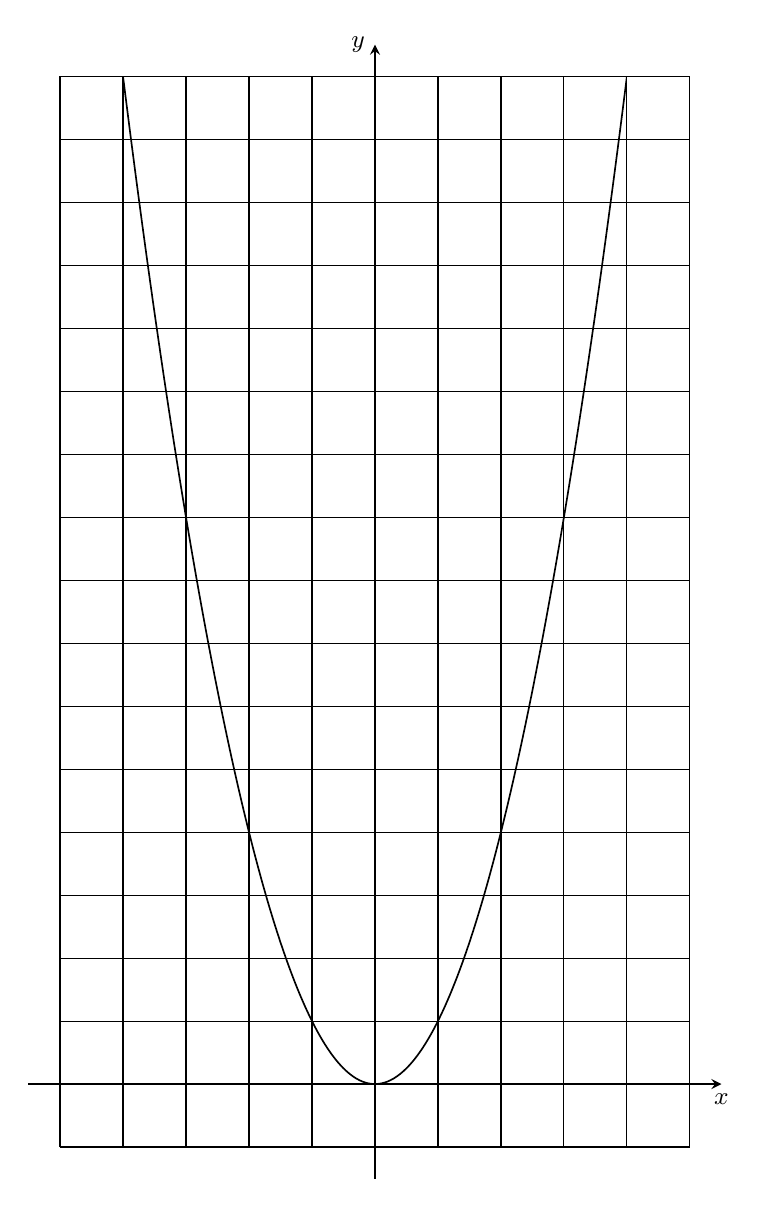
\begin{tikzpicture}[scale=0.8]
    \draw (-5, -1) grid (5, 16);
    \draw[line width=0.6pt, ->, >=stealth] (-5.5, 0) -- (5.5, 0) node[below]{{\small$x$}};
    \draw[line width=0.6pt, ->, >=stealth] (0, -1.5) -- (0, 16.5) node[left]{{\small$y$}};
    \begin{scope}
      \clip (-4.000, -0.050) rectangle (4.000, 16.000);
      \draw[line width=0.6pt] plot[smooth] coordinates
      {
        ( -4.000,  16.000)	        ( -3.900,  15.210)
        ( -3.800,  14.440)	        ( -3.700,  13.690)
        ( -3.600,  12.960)	        ( -3.500,  12.250)
        ( -3.400,  11.560)	        ( -3.300,  10.890)
        ( -3.200,  10.240)	        ( -3.100,   9.610)
        ( -3.000,   9.000)	        ( -2.900,   8.410)
        ( -2.800,   7.840)	        ( -2.700,   7.290)
        ( -2.600,   6.760)	        ( -2.500,   6.250)
        ( -2.400,   5.760)	        ( -2.300,   5.290)
        ( -2.200,   4.840)	        ( -2.100,   4.410)
        ( -2.000,   4.000)	        ( -1.900,   3.610)
        ( -1.800,   3.240)	        ( -1.700,   2.890)
        ( -1.600,   2.560)	        ( -1.500,   2.250)
        ( -1.400,   1.960)	        ( -1.300,   1.690)
        ( -1.200,   1.440)	        ( -1.100,   1.210)
        ( -1.000,   1.000)	        ( -0.900,   0.810)
        ( -0.800,   0.640)	        ( -0.700,   0.490)
        ( -0.600,   0.360)	        ( -0.500,   0.250)
        ( -0.400,   0.160)	        ( -0.300,   0.090)
        ( -0.200,   0.040)	        ( -0.100,   0.010)
        (  0.000,   0.000)	        (  0.100,   0.010)
        (  0.200,   0.040)	        (  0.300,   0.090)
        (  0.400,   0.160)	        (  0.500,   0.250)
        (  0.600,   0.360)	        (  0.700,   0.490)
        (  0.800,   0.640)	        (  0.900,   0.810)
        (  1.000,   1.000)	        (  1.100,   1.210)
        (  1.200,   1.440)	        (  1.300,   1.690)
        (  1.400,   1.960)	        (  1.500,   2.250)
        (  1.600,   2.560)	        (  1.700,   2.890)
        (  1.800,   3.240)	        (  1.900,   3.610)
        (  2.000,   4.000)	        (  2.100,   4.410)
        (  2.200,   4.840)	        (  2.300,   5.290)
        (  2.400,   5.760)	        (  2.500,   6.250)
        (  2.600,   6.760)	        (  2.700,   7.290)
        (  2.800,   7.840)	        (  2.900,   8.410)
        (  3.000,   9.000)	        (  3.100,   9.610)
        (  3.200,  10.240)	        (  3.300,  10.890)
        (  3.400,  11.560)	        (  3.500,  12.250)
        (  3.600,  12.960)	        (  3.700,  13.690)
        (  3.800,  14.440)	        (  3.900,  15.210)
        (  4.000,  16.000)
      };
    \end{scope}
  \end{tikzpicture}
\end{center}

% ------------------------------------------------------------------------------
\end{document}
% ------------------------------------------------------------------------------
